%%%% acra.tex
\documentclass{article} \usepackage{acra}

% Allow hyperlinks
\usepackage{hyperref}

% Allow using \linewidth
\usepackage{graphicx}

% Subcaption
\usepackage{subcaption}
\usepackage{caption}

% Allow float position for figures
\usepackage{float}

% Math tools
\usepackage{bm}
\usepackage{amsmath}
\usepackage[utf8]{inputenc}
\usepackage{siunitx}

\usepackage{array} % do i need this?
\usepackage{fourier} % do i need this?
\usepackage{makecell}

\renewcommand\theadalign{cl}
\renewcommand\theadfont{\bfseries}
\renewcommand\theadgape{\Gape[4pt]}
\renewcommand\cellgape{\Gape[4pt]}

\usepackage[labelfont=bf]{caption}

\title{Using Planar Point Correspondence to Calibrate Camera Arrays for Light
  Field Acquisition} \author{Ashley W. Stewart, Donald G. Dansereau
  \\ Queensland University of Technology, Australia; Stanford University
  \\ a.stewart.au@gmail.com, donald.dansereau@gmail.com}

\begin{document}

\maketitle

\begin{abstract}

  Light field cameras are an emerging technology with unique post-processing
  capabilities. For certain light field applications such as synthetic aperture
  photography, existing calibration procedures are either metric calibrations
  that are difficult to execute with low-cost hardware, or non-metric procedures
  that are inflexible to arbitrary sub-camera pose or require cameras with
  tightly controlled poses. We present a novel and comparatively simple
  non-metric procedure for light field acquisition that estimates the geometric
  transforms between camera images with respect to a calibration plane. The
  procedure is suitable for mobile camera arrays, and flexible to unknown or
  varied sub-camera pose. It only requires one image from each camera of a
  calibration pattern positioned to span the camera array's full field of
  view. We also provide a quantitative measure of calibration quality, and use
  it to demonstrate the procedure's efficacy with our Raspberry Pi camera
  array. The results highlight the procedure's robustness to variable camera
  orientation in contrast to existing state of the art techniques. Finally, we
  present qualitative results by rendering light fields at varying levels of
  focus and occlusion, and demonstrate success in capturing and rendering light
  field video.

\end{abstract}

\section{Introduction}

% Definition

\emph{Light fields} describe the amount of light flowing through space in all
directions. A light field \emph{camera} captures an array of views of a scene
using either an array of cameras \cite{yang2002real}, a lenslet array
\cite{ng2005light}, or a single camera on a controlled gantry
\cite{levoy_light_2006}. The resultant views are aligned using homographies so
that light rays can be identified via a two-plane parametrisation consisting of
a camera plane with cameras in $s,t$ and an image plane with pixels in $u,v$.

% Applications / importance WA

Some applications of light fields include image-based rendering
\cite{levoy_light_2006} and 3D geometry estimation
\cite{wanner2014variational}. Technologies such as 3D light field displays are
also emerging \cite{chen2014wide}. A popular application of light field cameras
is synthetic aperture photography \cite{levoy2004synthetic}, which involves
projecting images onto a focal plane and computing and rendering their average,
enabling post-capture refocussing. With a sufficiently wide synthetic aperture,
synthetic focussing can blur nearby occluders until they fade from view.

% Monocular calibration and why array calibrations are necessary

To achieve results in any such application, camera calibration is
essential. Calibration processes have been described for monocular cameras since
the early 1970s, first in photogrammetry \cite{duane1971close}, and later in
computer vision \cite{ganapathy_decomposition_1984}. Monocular camera
calibration involves estimating intrinsic and extrinsic camera parameters so
that images can be later rectified for accurate analysis and rendering. Early
light field capture was dominated by calibrated monocular cameras that travel
along controlled gantries. Although this technique allows the transformations
between viewpoints to be trivially calculated, it severely limits applications
outside the laboratory, and restricts capture to static scenes. Camera arrays
and lenslet arrays have greater potential, though finding the transformations
between viewpoints becomes non-trivial, especially when orientations differ. As
a result, calibrations for camera arrays and lenslet arrays have been developed
that recover sub-camera poses.

% How camera arrays are usually calibrated

Most camera array calibrations involve applying an extension to Zhang's
monocular calibration \shortcite{zhang2000flexible} across all viewpoints with
additional optimisation steps
\cite{ueshiba_planebased_2003,xumobile2014}. Calibrating camera arrays using
such processes is challenging, especially outside the laboratory and for mobile
arrays.

% Advantages of non-metric calibration

Vaish et al. \shortcite{vaish_using_2004} point out that for many light field
applications such as synthetic aperture photography, a metric calibration that
recovers camera parameters is unnecessary. Instead, only the relative positions
of viewpoints are needed to a scale to compute the projective transforms
necessary to render an image focussed at a given focal plane. Vaish achieves
this by measuring the parallax of several scene points across all cameras and
computing the nearest rank-1 factorization via Singular Value Decomposition
(SVD). This non-metric procedure was shown to produce better qualitative results
for synthetic aperture photography applications than those produced through
metric calibrations.

% Current limitations

Although Vaish's procedure is conceptually simple, it assumes that all camera
images are aligned at a reference plane. This allows scene point parallax in
images to be considered a function of relative camera position. Non-uniform
orientation among cameras voids this relationship as parallax becomes a function
of camera orientation in addition to position. This makes camera positions
irrecoverable by means of parallax measurement. This is a significant problem
for low-cost consumer cameras prone to inconsistent construction. Our Raspberry
Pi camera array, for example, was built to maintain front-facing orientations by
mounting cameras onto an aluminium plate, yet variable orientation is still
exhibited within their fixed camera boards.

\subsection{Contributions}

% Solution

We propose a novel calibration solution that recovers the geometric
transformations between images with respect to a calibration plane. Such
transformations are useful because they are a function of relative camera
\emph{pose} rather than \emph{position}. Our method can be achieved using only a
single image from all cameras of a calibration pattern spanning the camera
array's full field of view. Transformations are estimated using feature
detection and sample consensus algorithms. Another advantage of our solution is
that it largely relies on prevalent algorithms that already exist as standard
tools in most computer vision libraries, so implementing it requires few lines
of code.

% Other contributions

To support the use of our calibration, we also present a quantitative measure of
calibration quality. Vaish et al. \shortcite{vaish_using_2004} note that the
usual indicators of calibration accuracy such as reprojection error cannot be
measured for non-metric calibrations. Our measure of error is the total distance
between SURF feature points in calibration images after projecting them onto the
calibration plane using their estimated relative transformations. We have
achieved a significant improvement in SURF feature consistency from our
calibration compared to Vaish's. This will be true for any camera array with
variable camera orientation.

\section{Related Work}

Dansereau et al. \shortcite{dansereau_exploiting_2014} point out that image sets
suffering from parallax can be used to construct light fields by estimating the
geometric transformations between images and reprojecting them onto a common
plane. This is essentially what we have recognised and are taking advantage of
in our method. However, theirs requires an initial estimate of camera pose to be
known, parametrised by azimuths and elevations. This is possible when the pose
of cameras is tightly controlled, such as in their Ocular Robotics
\emph{RobotEye} camera system. The poses of our cameras are not tightly
controlled on their camera boards, so sub-camera poses cannot be recovered
without performing a metric calibration that estimates camera parameters.

Vaish et al. \shortcite{vaish_using_2004} also state that a possible area of
future work is investigating extensions to their technique for cameras in
general positions, as well as arbitrary reference planes using planar
homologies. Following this suggestion, we have identified a technique to align
camera images using planar point correspondence for cameras with variable
orientation.

\section{Calibration}

Consider a camera array consisting of cameras with unknown poses, and a
non-repeating planar calibration pattern positioned to span the array's full
field of view (see Figure \ref{fig:calibration_diagram}). The image set captured
in this scenario can be brought into focus at the calibration plane as a light
field by applying geometric transformations to the image set. Our approach will
estimate these transformations.

\begin{figure}[H] \centering
  \includegraphics[width=\linewidth]{images/calibration_diagram}
  \caption{Example calibration setup with camera plane on the left, and
    calibration plane on the right. Between the planes is the projection of two
    adjacent camera views with significant overlap. Our procedure requires that
    it be possible to position a calibration pattern that spans the array's full
    field of view with significant overlap between adjacent views.}
  \label{fig:calibration_diagram}
\end{figure}

\subsection{Choosing a Calibration Pattern}

The calibration pattern must be non-repeating so that erroneous feature matches
are minimised. This means that common calibration patterns such as checkerboards
are unsuitable. Additionally, the pattern must be sufficiently detailed so that
feature identification is strongly encouraged. Li et al.
\shortcite{li_multiple-camera_2013} have reverse engineered a pattern generator
that yields high quantities of detectable features using random noise. The
generator executes in multiple passes at varied scales so that plentiful
features can be detected at a range of distances. Calibration patterns generated
this way are suitable. We have also achieved good results using certain detailed
paintings and posters. Though results may vary using paintings and posters, it
is a convenient alternative to printing a potentially large pattern.

\subsection{Transform Estimation and Image Rectification}

Once a calibration image has been captured by each camera, feature matching can
begin. We identify features across all views using Speeded-Up Robust Features
(SURF) \cite{bay2008speeded}. This generates a point matrix and a feature
descriptor matrix for each image. Unique, matching points between adjacent image
pairs are then collected if the error between feature vectors is within a
threshold. Not all image pairs need to be compared; we compare only successive
and adjacent image pairs (i.e. with an image set $\bm{I}$, we match features in
$I_0\leftrightarrow{}I_1,I_1\leftrightarrow{}I_2,...$). The sets of points
matched between each successive image pair become the main inputs into the
Maximum Likelihood Estimation SAmple Concensus algorithm (MLESAC)
\cite{torr2000mlesac}, which provides an initial set of geometric
transformations. MLESAC uses the same strategy as the more common RANSAC
\cite{fischler1981random}, but chooses solutions according to maximum likelihood
rather than the number of inliers, overcoming non-linear constraints between
parameters.

% Accounting for distortion

The transformations returned by MLESAC will be relative to the first camera's
image, causing a progressive distortion of the later images. This can be
resolved by choosing an alternative image as the anchor and applying its inverse
transform to all the others, so that the anchor image becomes the least
distorted. We measure the $u,v$ limits of each image after projecting them onto
the calibration plane via their estimated transforms to identify the central
image and use it as the anchor. Choosing the central image as the anchor will
reduce overall distortion.

The final set of transformations can be used to rectify any image set captured
by the array into light field alignment at the calibration plane.

\subsection{Synthetic Aperture Focussing}

If relative camera positions are known, then images can be translated into
alignment at any plane parallel to the calibration plane for synthetic
focussing. With a desired focal depth $d$ relative to the calibration plane, and
cameras with relative positions in $\bm{\Delta P}$, each camera image $C_i$
should each be translated by $-d\Delta P_i$ to bring them into alignment
\cite{vaish_using_2004}. Results are rendered by taking the average of all
translated images.

% maybe remove
% If relative camera positions are unknown, they may be estimated by first
% aligning unrectified calibration images to a common scene point near the array's
% principal axis, and applying Vaish's plane + parallax procedure on a range of
% scene points. This may provide acceptable results if cameras on average have the
% same orientation as the array.

\section{Implementation and Results}

Our Raspberry Pi camera array uses Raspberry Pi V1 camera modules arranged in a
4x4 grid (see Figure \ref{fig:rpi_camera_array}). Their orientations are
unknown, though they are known to be non-uniform. Our cameras are approximately
planar and evenly spaced.

\begin{figure}[H] \centering
  \includegraphics[width=0.8\linewidth]{images/rpicam}
  \caption{Our Raspberry Pi Camera Array}
  \label{fig:rpi_camera_array}
\end{figure}

Although we suggest using a calibration pattern generated via noise functions
\cite{li_multiple-camera_2013}, we demonstrate the flexibility of our solution
by using an image of a painting displayed on a TV positioned 300mm in front of
the camera array. The painting used is Leonid Afremov's \emph{Farewell to
  Anger}. Our horizontal and vertical sub-camera fields of view are
$\phi=(\ang{53.5}, \ang{41.41})$, and distances between cameras are each roughly
34mm. This makes our horizontal and vertical $u,v$ overlaps on the calibration
plane approximately 89\% and 85\%.

% maybe remove
% To produce synthetic focussing results, relative camera positions must be
% known. Ours are known to be equal, but they can be estimated by bringing
% unrectified images of a scene into alignment at a point by translation only, and
% applying Vaish's \emph{Plane + Parallax} procedure to estimate camera positions
% through parallax measurement \shortcite{vaish_using_2004}. For completeness, we
% performed this and computed camera positions with a mean error of 0.51mm $\pm$
% 0.45mm, but continued with their known values.

Our qualitative results include focussed light field stills, including
animations of stills in which the level of focus varies between planes of
interest (see Figure \ref{fig:focussing_demo}). Notice that the objects in the
focal plane are clear, while the objects elsewhere appear blurred, and occluders
fade from view when the focus is on the background. Clear focus levels are
indicative of a high quality calibration.

We have also captured light field video of indoor and outdoor scenes
with panning focus and moving objects (see Figure \ref{fig:video_screens}). Our
synthetic focussing results and robustness to occluders compares well with the
results others have achieved using similar procedures.

\newpage

\begin{figure}[H] \centering
  \begin{subfigure}[b]{0.95\columnwidth}
    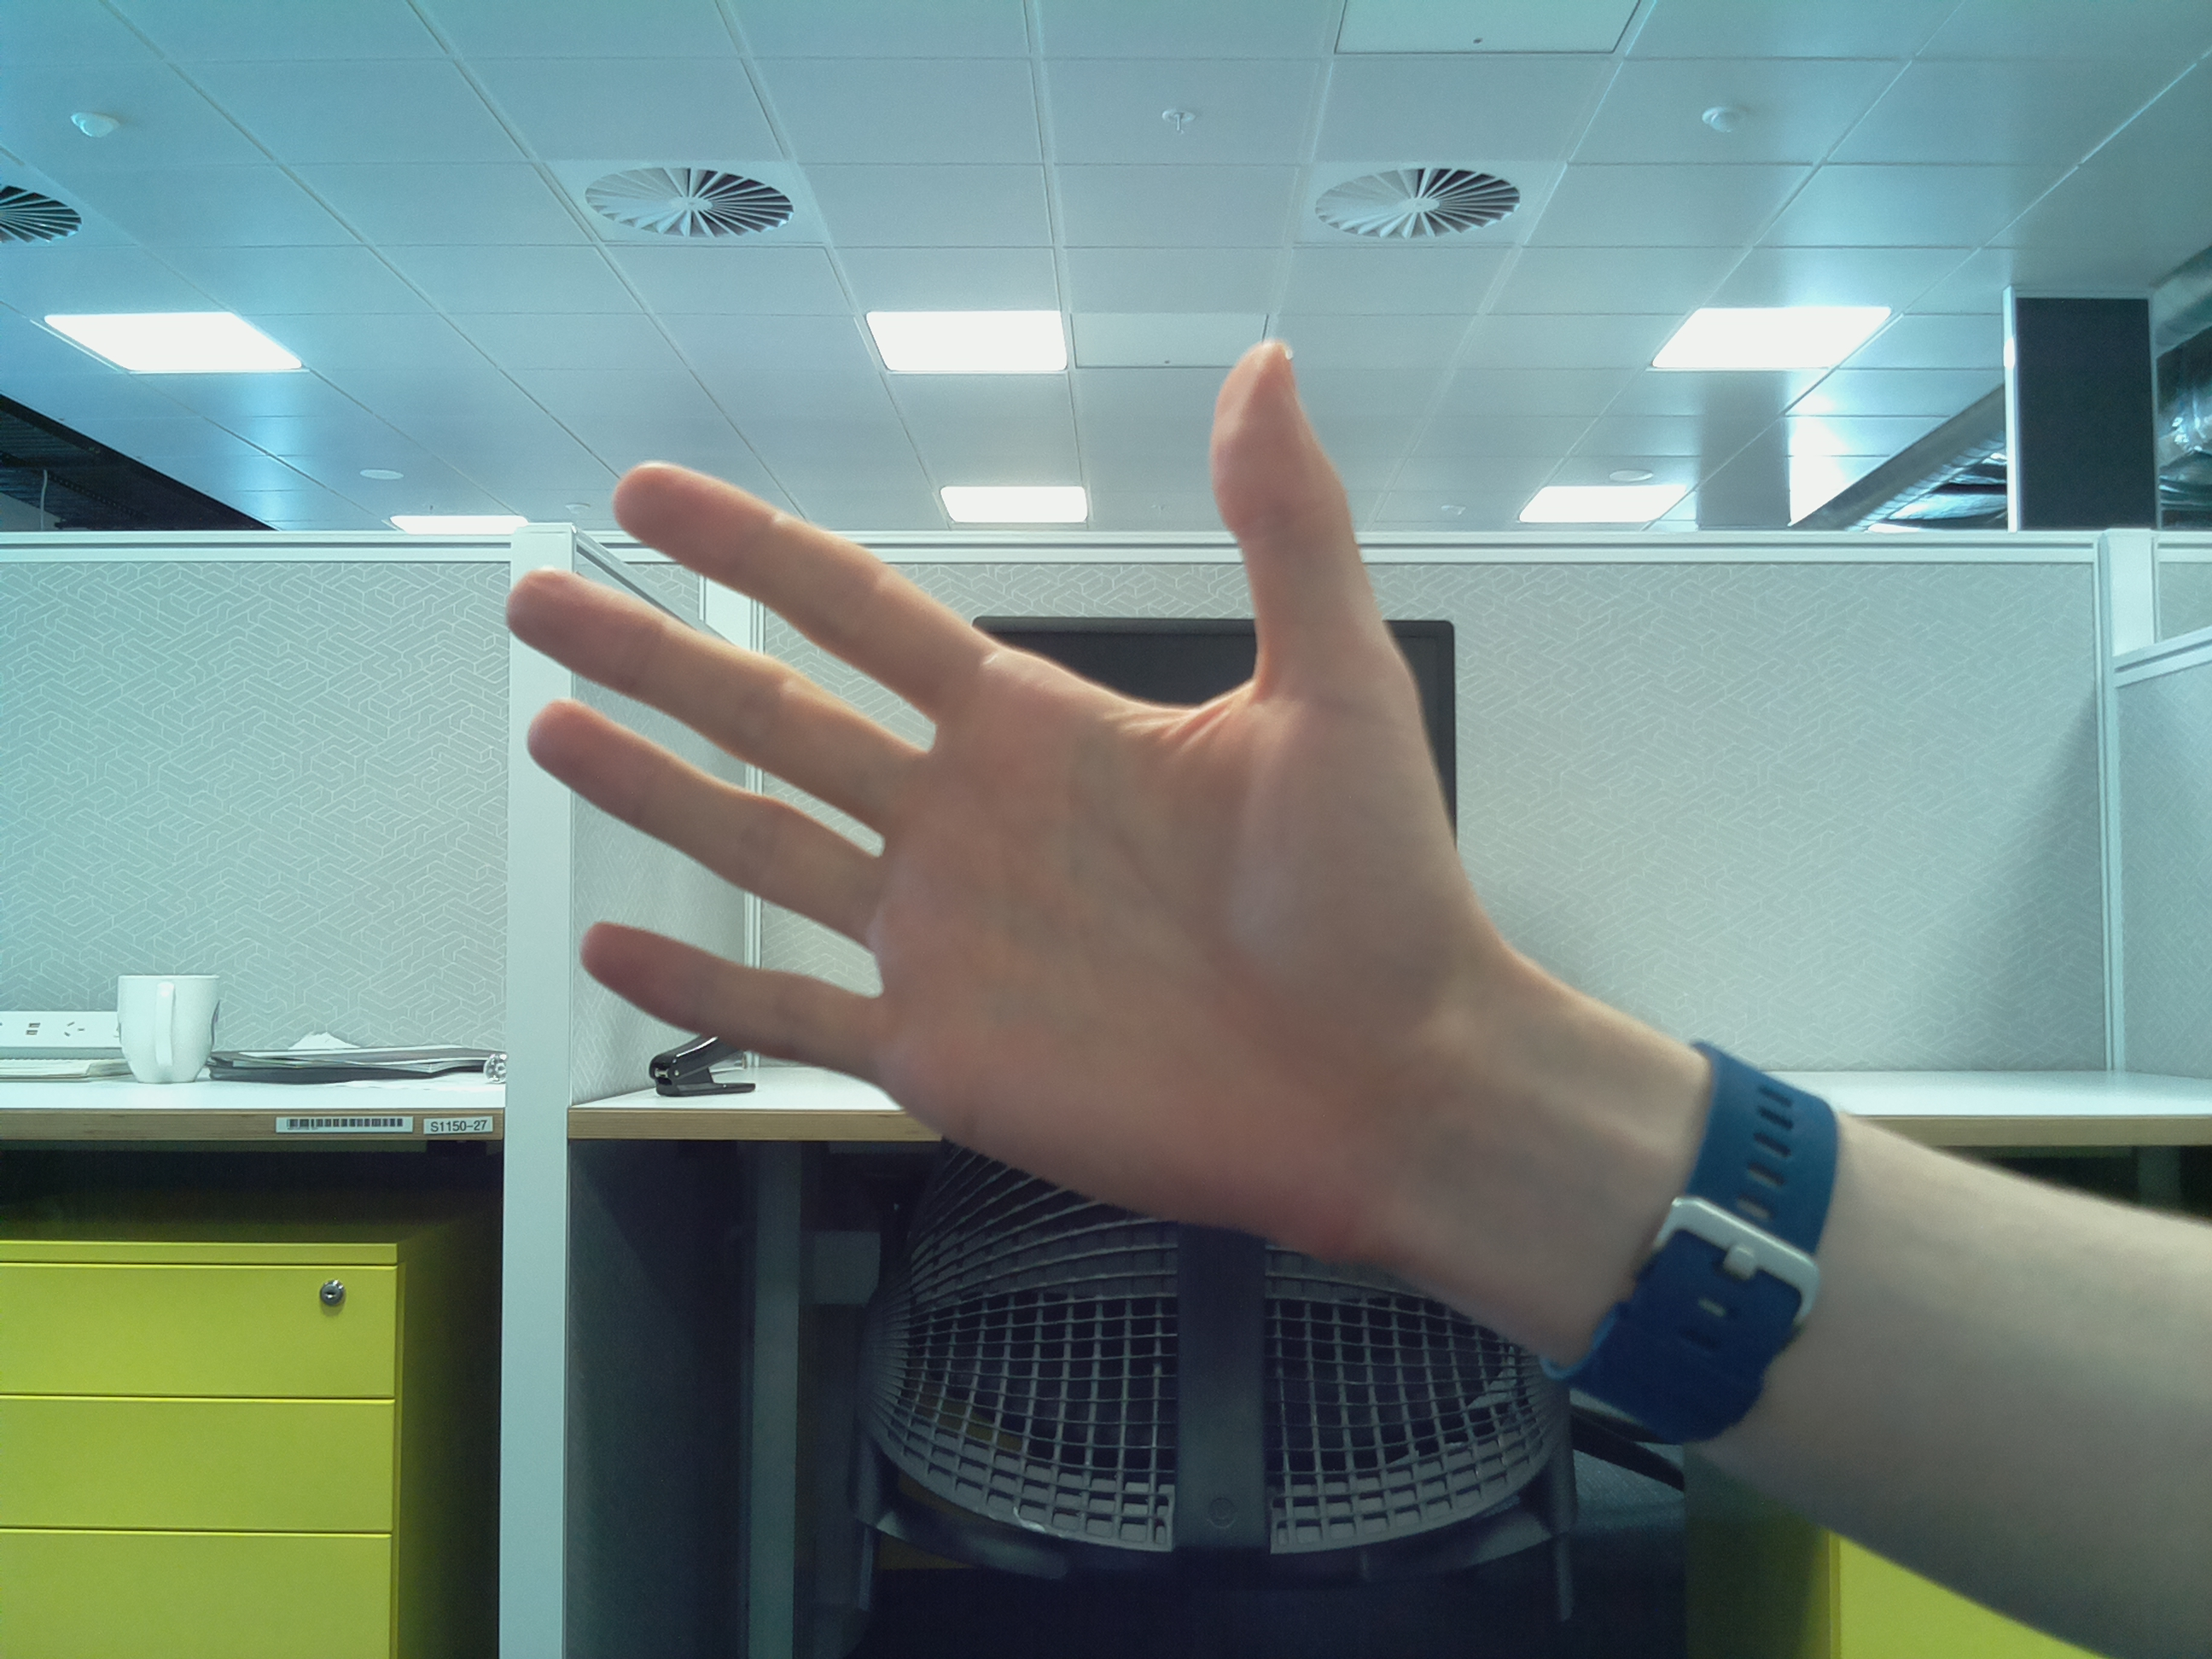
\includegraphics[width=\columnwidth]{images/focussing_demo_c}
    \caption{Unrectified image from one of the Raspberry Pi V1 camera modules}
  \end{subfigure}
  \begin{subfigure}[b]{0.95\columnwidth}
    \includegraphics[width=\textwidth]{images/focussing_demo_d}
    \caption{Light field focussed on the office chair in the background}
  \end{subfigure}
  \begin{subfigure}[b]{0.95\columnwidth}
    \includegraphics[width=\textwidth]{images/focussing_demo_b}
    \caption{Light field focussed on the occluding hand in the foreground}
  \end{subfigure}
  \caption{Rendered light field still demonstration displaying an office scene
    at two levels of focus with an occluding hand (focus animations available
    online) \protect\cite{stewart2017using}}
  \label{fig:focussing_demo}
\end{figure}

\begin{figure}[H] \centering
  \begin{subfigure}[b]{0.73\columnwidth}
    \includegraphics[width=\textwidth]{images/vid_4}
    \caption{Video 1, background in focus}
  \end{subfigure}
  \begin{subfigure}[b]{0.73\columnwidth}
    \includegraphics[width=\textwidth]{images/vid_3}
    \caption{Video 1, foreground in focus}
  \end{subfigure}
  \begin{subfigure}[b]{0.73\columnwidth}
    \includegraphics[width=\textwidth]{images/vid_2}
    \caption{Video 2, background in focus}
  \end{subfigure}
  \begin{subfigure}[b]{0.73\columnwidth}
    \includegraphics[width=\textwidth]{images/vid_1}
    \caption{Video 2, foreground in focus}
  \end{subfigure}
  \caption{Screenshots from some of our light field videos (full videos
    available online) \protect\cite{stewart2017using}}
  \label{fig:video_screens}
\end{figure}

To qualitatively demonstrate the effectiveness of applying relative view
transformations to handle non-uniform orientation, we compare the visual clarity
of synthetic focussing results rendered with no alignment, alignment by
translation only, and alignment by transformation (see Figure
\ref{fig:visual_comparison}). No alignment is akin to to applying Vaish et al.'s
calibration, ignoring varied camera orientation. We compare our results with
Vaish even though their method is not well suited to our implementation, because
it is the only other non-metric calibration that we are aware of. Alignment by
translation is a more primitive version of our technique that applies only
translations to align images at a point. The results highlight the benefits of
applying the more complete transformations recovered by our procedure.

\begin{figure}[h] \centering
  \includegraphics[width=\columnwidth]{images/comparison}
  \caption{Close-up of synthetic focussing results using three rectification
    techniques. Notice the progressive increase in visual clarity, the best of
    which was achieved by our geometric transformation method.}
  \label{fig:visual_comparison}
\end{figure}

We obtain quantitative results by measuring the pixel distance between matching
SURF features in calibration images projected onto the calibration plane. This
provides a reliable measure of focal error. We compare the results of the same
three rectification techniques as in our qualitative comparison (see Figure
\ref{fig:boxplot}).

\begin{figure}[h] \centering
  \includegraphics[width=\columnwidth]{images/boxplot-pixelerror}
  \caption{Positional error of SURF features measured in an image set for three
    rectification techniques. Notice the progressive decline in error, the
    lowest of which was achieved by our geometric transformation method.}
  \label{fig:boxplot}
\end{figure}

We found that running multiple passes of our procedure yields more precise view
transformations. Multiple passes can be executed by running the procedure
successive times against the rectified calibration set. For our setup, two
passes yield a significant improvement, with diminishing returns achieved
thereafter (see Table \ref{tbl:pixel-inconsistencies}).

\begin{table}[h] \centering

  \caption{Feature error across our aligned calibration images after several
    calibration passes.}

  %\resizebox{\columnwidth}{!}{
    \begin{tabular}{l|l|l}

      \thead{Pass \\ \#} &
      \thead{Average \\ $\bm{u}$-feature error \\ (pixels)} &
      \thead{Average \\ $\bm{v}$-feature error \\ (pixels)} \\

      \hline % horizontal line
                                                              
      1 & 5.092 & 5.155 \\
      2 & 1.178 & 0.884 \\
      3 & 1.184 & 0.917 \\
      4 & 1.160 & 0.925

    \end{tabular}
 % }
    
  \label{tbl:pixel-inconsistencies}
\end{table}


\section{Conclusions and Future Work}

As research in light field technology has progressed and applications have
expanded, so too has the need for robust calibrations. Our calibration procedure
can be carried out with camera arrays constructed with low-cost hardware. It is
also exceptionally robust; the only restriction on the camera array itself is
that it must be possible to position a calibration pattern that spans its full
field of view, and that sufficient features can be detected and matched between
images. Our calibration is also remarkably easy to implement, with most of the
processes needed (SURF, MLESAC, and noise generators) already built into current
standard computer vision libraries and tools such as OpenCV and MATLAB.

Our qualitative aperture focussing results compare well with those achieved
using similar, non-metric calibrations. Vaish et
al. \shortcite{vaish_using_2004} have also shown that non-metric calibrations
that minimise parallax on a reference plane produce better qualitative results
than metric calibrations. Our quantitative results highlight our procedure's
robustness to non-uniform orientation.

Finally, we also demonstrate the capture and rendering of light field video
using low-cost hardware. Currently, little work has been done on light field
technology that exploits or identifies the unique properties of the temporal
axis. Our calibration enables even the most entry-level technology to be used in
this exciting area. Work in synthetic aperture photography, for instance, shows
that objects can be tracked in light field video through dense occluders
\cite{joshi2007synthetic}.

\section*{Acknowledgements}

We would like to express our gratitude to the Australian Research Council Centre
of Excellence for Robotic Vision for supporting this project (project number
CE140100016). We would also like to extend a special thanks to Rafe Denham for
his work on the camera array, and finally to Steven Martin for his assistance in
capturing outdoor light field video, and for his alterations to the camera
array.

\bibliography{acra}{}
\bibliographystyle{named}

\end{document}
